\documentclass{article}
\usepackage{amsmath}
\usepackage{graphicx}
\usepackage{bm}
\usepackage{pdfpages}

\newcommand{\bra}[1]{\langle#1|}
\newcommand{\ket}[1]{|#1\rangle}

\begin{document}

\title{Untangling hyperfine level malarkey}
\date{}
\maketitle

\section{Context}

Figure \ref{data_peaks} shows absorption peaks for laser light to helium at frequencies denoted by the x-axis in a DC magnetic field of strength 11G and 18G (blue and red respectively). The atom is initially in the $m_J = 2$ state of the $2^3P_2$ level.


These lines are identified as transitions to the $5^3D_2$ and $5^3D_3$ levels. We also have measured frequencies for the $2^3P_2\rightarrow5^3D_1$ transition in both background fields. The problem statement is: \emph{Given} the experimentally measured peak frequencies and \emph{assuming} the quantum mechanical description of the atom, \emph{determine} the absolute frequencies of the $2^3P_2\rightarrow 5_D$ transitions in the unperturbed helium atom. The outcome is currently a partial solution, and an indication of what is needed to reach a more complete solution.

\begin{figure}[h]
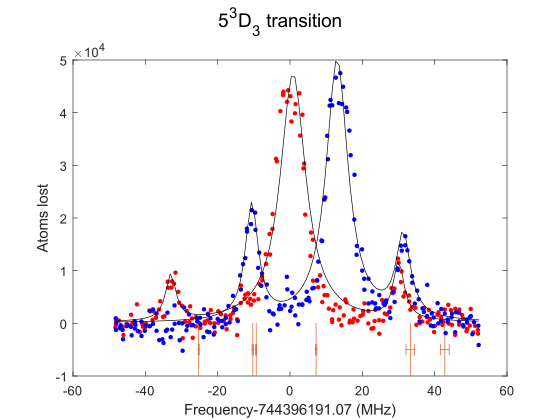
\includegraphics[width=\textwidth]{figs/5^3D_3_plot_combo.png}
\label{data_peaks}
\caption{Beautiful peaks, look at them shine}
\end{figure}

\subsection{Old method}
Previously, I used a linear fit to the peak values as a function of field strength to extrapolate to the zero-field values. This isn't horrifically wrong but it is incorrect because for small field values, there is a nonlinear shift in the closely-spaced energies of the $D_2$ and $D_3$ levels, as explained below. Therefore one must use Actual Theory to work obtain the field-free transition energies.

I asked Danny for some assistance here, and what follows is an extension of the background material he provided.

\section{Identifing peaks}



Figure \ref{theory_plots} shows the frequencies of the transitions to the $J=2$ and $J=3$ levels, relative to the zero-field $J=3$ level, as a function of field strength assuming a 21MHz splitting between the bare levels. Shown are the $m_j$ = 1 (black), 2 (blue), and 3 (red) lines from each level (the $J=3$ being the lowest). Notice that at 11G and 18G, the experimentally relevant fields, the $|J,m_J\rangle = |3,2\rangle$ and $|J,m_J\rangle = |2,1\rangle$ lines are very close, or even intersecting. In the red spectrum in figure 1, one can just make out two distinct peaks in the central peak. We conclude that the larger central peak in both spectra is the coincidence of the two transitions. Checking the metadata for this experimental run confirms that the waveplate was set at an angle such that some $\pi$ light was present, which is different from the other measured spectra (not shown here). 

The question now is to determine the zero-field value of the fine structure splitting. We will use the smaller extremal peaks, the $|J,m_J\rangle = |3,1\rangle$ and $|J,m_J\rangle = |2,2\rangle$ lines, for this calculation as they are sufficiently distinct. The peak separation depends on the zero-field splitting and the magnetic field strength. By fixing the latter we can constrain the former. By minimizing the squared difference between the predicted and measured interval $f_{|3,1\rangle}-f_{|2,2\rangle}$, we constrain the splitting. Figure 2b. shows the squared error as a function of splitting value, which is minimized at 21MHz, 2MHz larger than the 19MHz prediction given in Wiese and Fuhr. 

This does not, unfortunately, give us the absolute frequency of these levels. In this calculation, the $J=1-J=3$ interval was assumed to be 315 MHz (actually larger than the predicted 303MHz, but the interference from a peak this far away should be small). In the next part I suggest a few ways forward.

\begin{figure}
\includegraphics[width=\textwidth]{figs/theory_splitting_work.png}
\label{theory_plots}
\caption{Theoretical lines as a function of magnetic field strength for fixed splitting, and the sum-square error of the predicted $f_{|3,1\rangle}-f_{|2,2\rangle}$, summed over measurements at both field values, versus the fine structure splitting.}
\end{figure}

\section{Determination of the absolute transition frequencies}

The current methods allow us to determine the fine structure splitting between the $J=2$ and $J=3$ levels of the helium $5^3D$ manifold (Are those terms right?). Determining the absolute frequency will require additional intervals. Up until now, the $J=3-J=1$ interval was input to the calculations. This is circular, assuming the theory we are trying to test. We would do better to use our experimental data and the quantum theory of the atom to work backwards to the field intervals. We could do this by extending the treatment above with a three-parameter fit - the absolute frequency of the $J=1$ transition, and the fine structure intervals (or, equivalently, the absolute frequencies of each transition), fitting to all available peaks as listed in table \ref{peaktable}. 

\section{Extending work}

Whereas previously we just used the CG coefficients givin the $\bra{Jm_J}$ basis in terms of the $\bra{m_L m_S}$ basis, using only the $m_J=1$ subspace, we now need to extend this to the $m_J=2$ and $m_J=3$ subspace. This is just a matter of writing some bigger matrices, but involves calculating/looking up more CG coefficients.

(remember the $\ket{\alpha}$ basis is the $\ket{Jm_J}$ basis and the $\ket{\beta}$ basis is the $\ket{m_Lm_S}$ basis.)

So we want to work in the subspace spanned by 
\begin{equation}
	\bm{\alpha} = \{\ket{11},\ket{21},\ket{22},\ket{31},\ket{32}\}
\end{equation}

We also have one (bad) measurement which includes the $\ket{33}$ line but we don't talk about that.

What's the basis we want to project back on to, then? The $\ket{\beta}$ basis, subject to $m_L+m_S=m_J$.
In the upper state, $L=2$ so $m_L\in\{-2,-1,0,1,2\}$ and $m_S\in\{-1,0,1\}$ right? 
and $m_J\in\{1,2\}$.

\begin{equation}
	\bm{\beta} = \{\ket{01},\ket{10},\ket{11},\ket{2-1},\ket{20}\}
\end{equation}

Ok great, now just need to look up the CG coefficients! And can look at Danny's work to confirm. U transforms the $m_L m_S$ basis into the $J m_J$ basis. 
% We have L = j1 = 2, S = j2 = 1 (angular and spin momenta)
% And the coefficients are: m_L = 2 1 or 0, m_S = -1 0 or 1

% j=1 m=1 
% mL mS CG
% 2 -1 \sqrt{3/4)
% 1 0 -\sqrt{3/10)
% 0 1 \sqrt{1/10)

% j=2 m=1
% mL mS CG
% 2 -1 \sqrt{1/3)
% 1 0 \sqrt{1/6)
% 0 1 -\sqrt{1/2)

% j=2 m=2
% mL mS CG
% 2 0 \sqrt{2/3)
% 1 1 -\sqrt{1/3)

% j=3 m=1
% mL mS CG
% 2 -1 \sqrt{1/15)
% 1 0 \sqrt{8/15)
% 0 1 \sqrt{2/5)

% j=3 m=2 
% mL mS CG
% 2 0  \sqrt{1/3)
% 1 1 \sqrt{2/3)
H\alpha = \mu_B/\hbar B (m_L+2m_s)

U is:
\begin{equation}
\begin{bmatrix}
% 01		  	10					11			2-1			20
\sqrt{1/10} &-\sqrt{3/10}	&   0		&  \sqrt{3/5}	&    0	\\ %\J mJ = 11
-\sqrt{1/2}	& \sqrt{1/6}	&	0 		&  \sqrt{1/3}	&    0	\\ %\J mJ = 21
	0		&	0			&-\sqrt{1/3}&  	0  			&   \sqrt{2/3} 	\\ %\J mJ = 22
\sqrt{2/5}  &	\sqrt{8/15}	&	 0		&  \sqrt{1/15}  &    0 	\\ %\J mJ = 31
	0		&	0			&\sqrt{2/3} &  0   			&    \sqrt{1/3}	\\ %\J mJ = 32
\end{bmatrix}
\end{equation}
\begin{table}
\label{peaktable}
\begin{tabular}{|c c|c|c|}
\hline
Line & Field & Peak centre & peak width\\
\hline
$5^3D_{1}$ & $|B| = 18G$& 744396451.51(0.10) MHz & 6.43(0.29) MHZ\\
			& $|B| = 11G$& 744396475.92(0.12) MHz & 5.15(0.33) MHZ\\
\hline
$5^3D_{2,3}$ & $|B| = 18G$& 744396158.56(0.21) MHz & 3.44(0.55) MHZ\\
						&& 744396191.07(0.16) MHz & 8.56(0.49) MHZ\\
						&& 744396221.11(0.16) MHz & 3.67(0.44) MHZ\\
			& $|B| = 11G$& 744396180.50(0.14) MHz & 4.34(0.40) MHZ\\
						&& 744396204.54(0.13) MHz & 7.33(0.39) MHZ\\
						&& 744396222.65(0.16) MHz & 4.75(0.47) MHZ\\
\hline
\end{tabular}
\caption{Relevant measured peak frequencies}
\end{table}




\appendix
\includepdf[pages=-]{doc/20200218_danny_theory_1}

\end{document}